\begin{tikzpicture}
% comment it out at the end
%\draw[help lines] (0,0) grid(20,20);

% STS rectangle
\coordinate (TLSTS) at (4,16);
\coordinate (BRSTS) at (12,12) {};

% LTS rectangle
\coordinate (TLLTS) at (4,10);
\coordinate (BRLTS) at (12,6);

% Data feeder rectangle
\coordinate (TLDF) at (0,15);
\coordinate (BRDF) at (2,13) {};

% Draw rectangles and their names in corners
\draw [ultra thick, rounded corners, blue] (TLSTS) rectangle (BRSTS);
\draw [ultra thick, rounded corners, blue] (TLLTS) rectangle (BRLTS);
\node [below right] at (TLSTS) {Short Term Smoother};
\node [below right] at (TLLTS) {Long Term Smoother};

% Draw Vision feeder
\draw [ultra thick, rounded corners, blue] (TLDF) rectangle (BRDF);
\node [below right] at (TLDF) {Data input};

% Draw data flow

\draw [ultra thick, ->] ($(BRDF) + (0,1)$) -- ($(TLSTS) - (0,2)$);
\draw [ultra thick, ->] ($(BRDF) + (0,1)$) -- ($(BRDF) + (1,1)$)
  -- ($(BRDF) + (1,-5)$) --  ($(TLLTS) - (0,2)$);


\draw [ultra thick, ->] ($(TLSTS)+(2,-4)$) -- ($(TLLTS)+(2,0)$);
\draw [ultra thick, ->] ($(TLLTS)+(6,0)$) -- ($(TLSTS)+(6,-4)$);

% node [right] {Pose estimates};

% TODO not a nice solution to include the pdf
\node at (8.5,14) {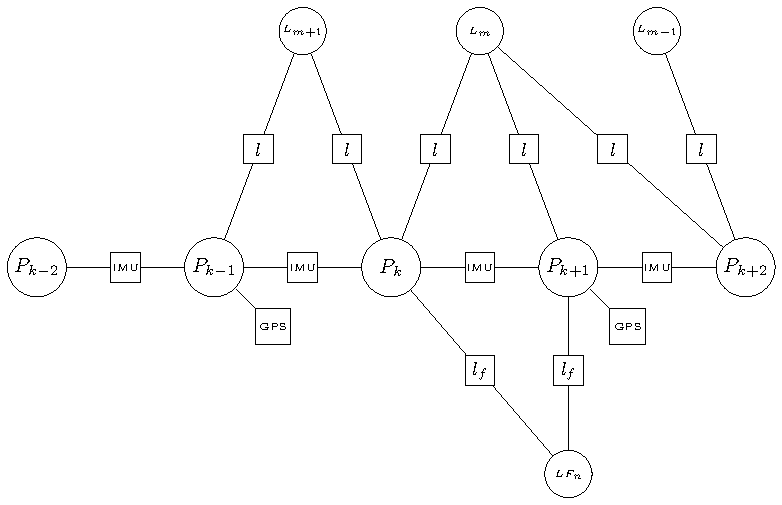
\includegraphics[scale=0.4]{./../factor_graph/factor_graph.pdf}};
\node at (9,8) {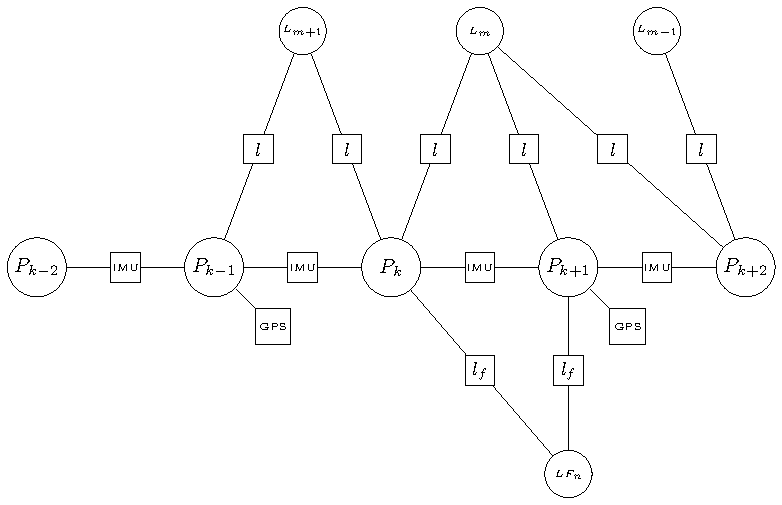
\includegraphics[scale=0.35]{./../factor_graph/factor_graph.pdf}};


%% TODO add it below \end
%\caption{Do not forget!
%Make it explicit enough that readers
%can figure out what you are doing.}

\draw [ultra thick, rounded corners, purple] (5.5,8.5) ellipse (0.5 and 0.2);
\node (v1) at (5,7.1) {};
\node (v2) at (5,8.6) {};
\node (v3) at (6,8.6) {};
\node (v4) at (6,7.1) {};
\draw [ultra thick, rounded corners, purple] (v1) edge (v2);
\draw [ultra thick, rounded corners, purple] (5,7.25) arc (180:360:0.5 and 0.2);
\draw [ultra thick, rounded corners, purple] (v3) edge (v4);

\node at (5.5,7.75) {Map};

\end{tikzpicture}


    
    
    